\documentclass{../../tex_template/asaproc}
\usepackage{graphicx} % \includegraphics
\usepackage{float}    % To keep figures in right place. 
                      % Usage: \being{figure}[H] \includegraphics{tmp.pdf} \end{figure}
\usepackage{subfig}   % \subfloat
\usepackage{amsmath}  % bmatrix, pmatrix, etc
\usepackage{bm}
\newcommand{\p}[1]{\left(#1\right)}
\newcommand{\bk}[1]{\left[#1\right]}
\newcommand{\bc}[1]{ \left\{#1\right\} }
\newcommand{\abs}[1]{ \left|#1\right| }
\newcommand{\E}{ \text{E} }
\newcommand{\N}{ \mathcal N }
\newcommand{\ds}{ \displaystyle }

%\usepackage{times}
%If you have times installed on your system, please
%uncomment the line above

%For figures and tables to stretch across two columns
%use \begin{figure*} \end{figure*} and
%\begin{table*}\end{table*}
% please place figures & tables as close as possible
% to text references

\newcommand{\be}{\begin{equation}}
\newcommand{\ee}{\end{equation}}

\title{Quiz 2 --- EU referendum poll tracker}

%input all authors' names
\author{
  Arthur Lui$^1$\\
  University California -- Santa Cruz$^1$\\
}

%input affiliations
%{USDA Forest Service Forest Products Laboratory}

\begin{document}
\maketitle
\begin{abstract}

\begin{keywords}
Lasso, Bayesian lasso, EU, regression, phone polls
\end{keywords}
\end{abstract}

\section{Introduction}

%\ref{fig:pairs}
\begin{figure}[H]
  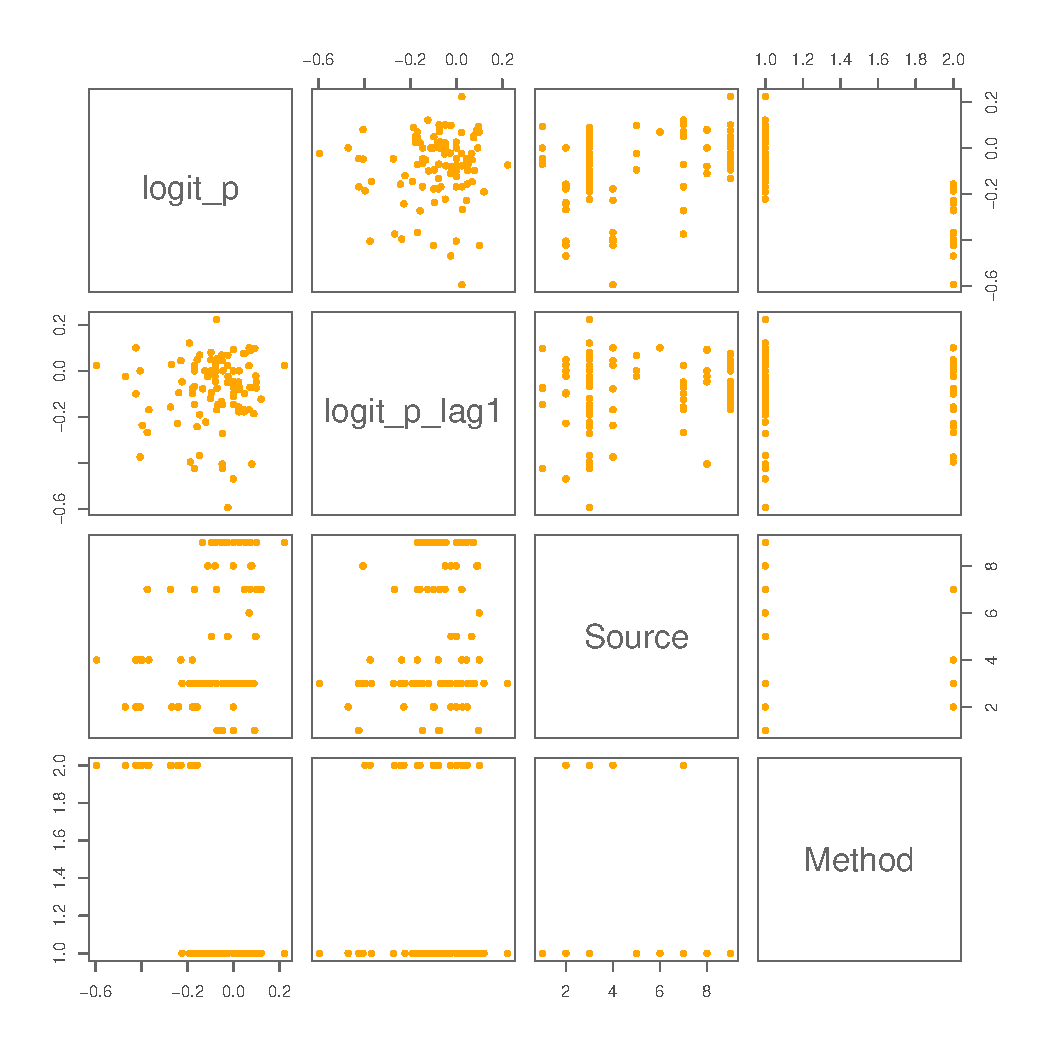
\includegraphics[scale=.5]{figs/pairs.pdf}
  \caption{\small Scatter plot matrix of (1) logit($p$), where $p$ is the
    number of people in facor of leaving the EU over the sum of the number of
    people in favor of leaving the EU and the number of people in favor of
    remaining in the EU; (2) logit(p) with a lag of 1 time period; (3) Syrvey
    Source which is one of Survation, ICM, Opinium, YouGov, ComRes, Ipsos Mori,
    TNS, BMG, or Panelbase; (4) Surveying Method: Phone or Online.}
  \label{fig:pairs}
\end{figure}

\begin{figure}[H]
  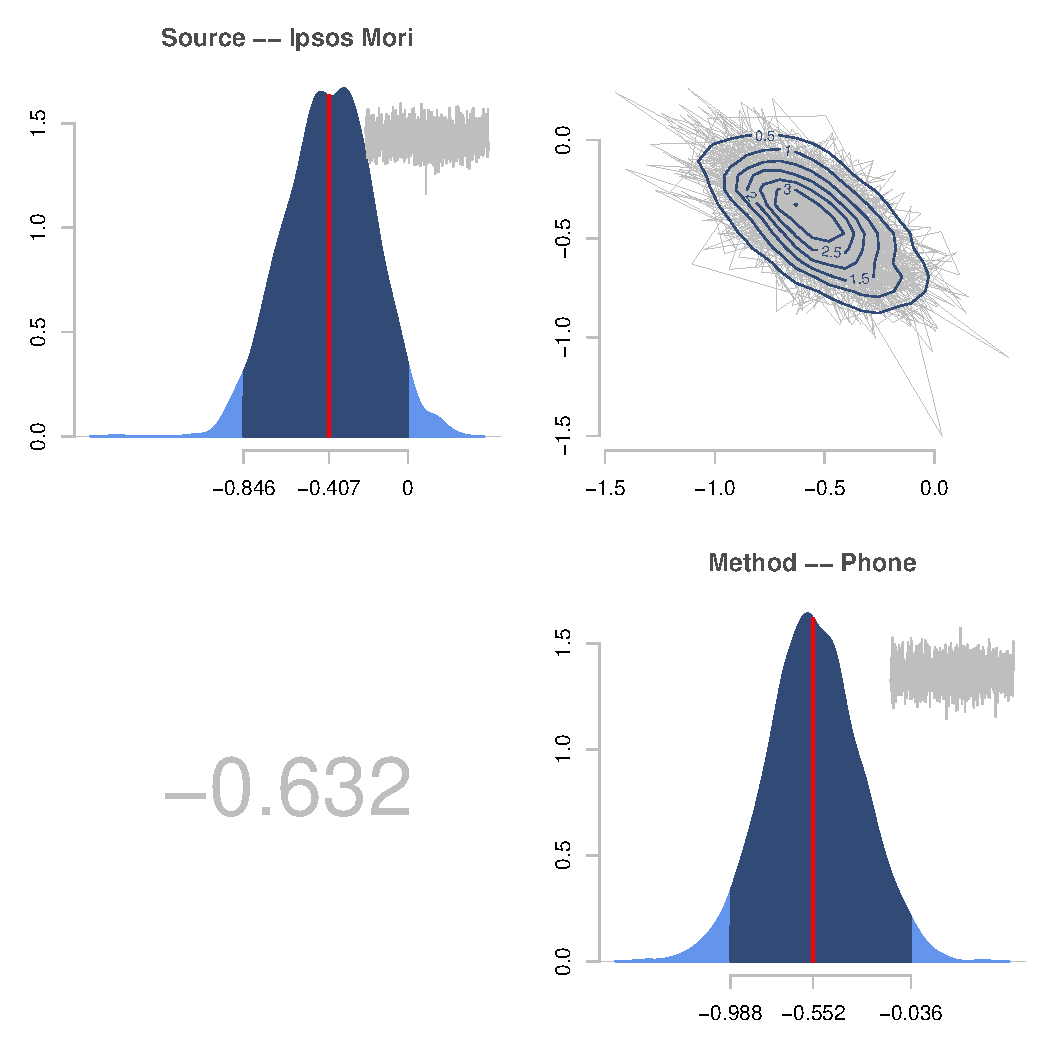
\includegraphics[scale=.5]{figs/posts.pdf}
  \caption{\small }
  \label{fig:posts}
\end{figure}

\begin{figure}[H]
  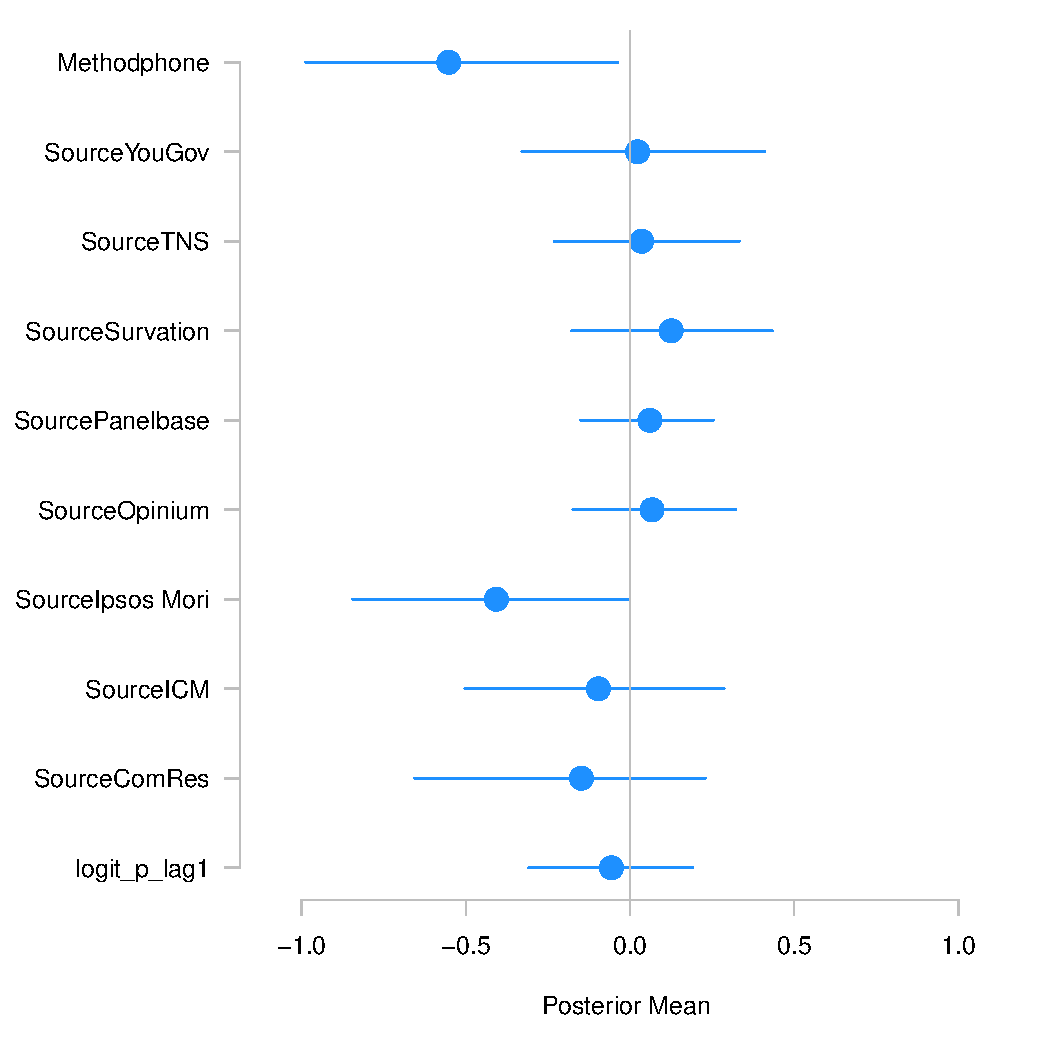
\includegraphics[scale=.5]{figs/allposts.pdf}
  \caption{\small }
  \label{fig:allposts}
\end{figure}

\begin{figure}[H]
  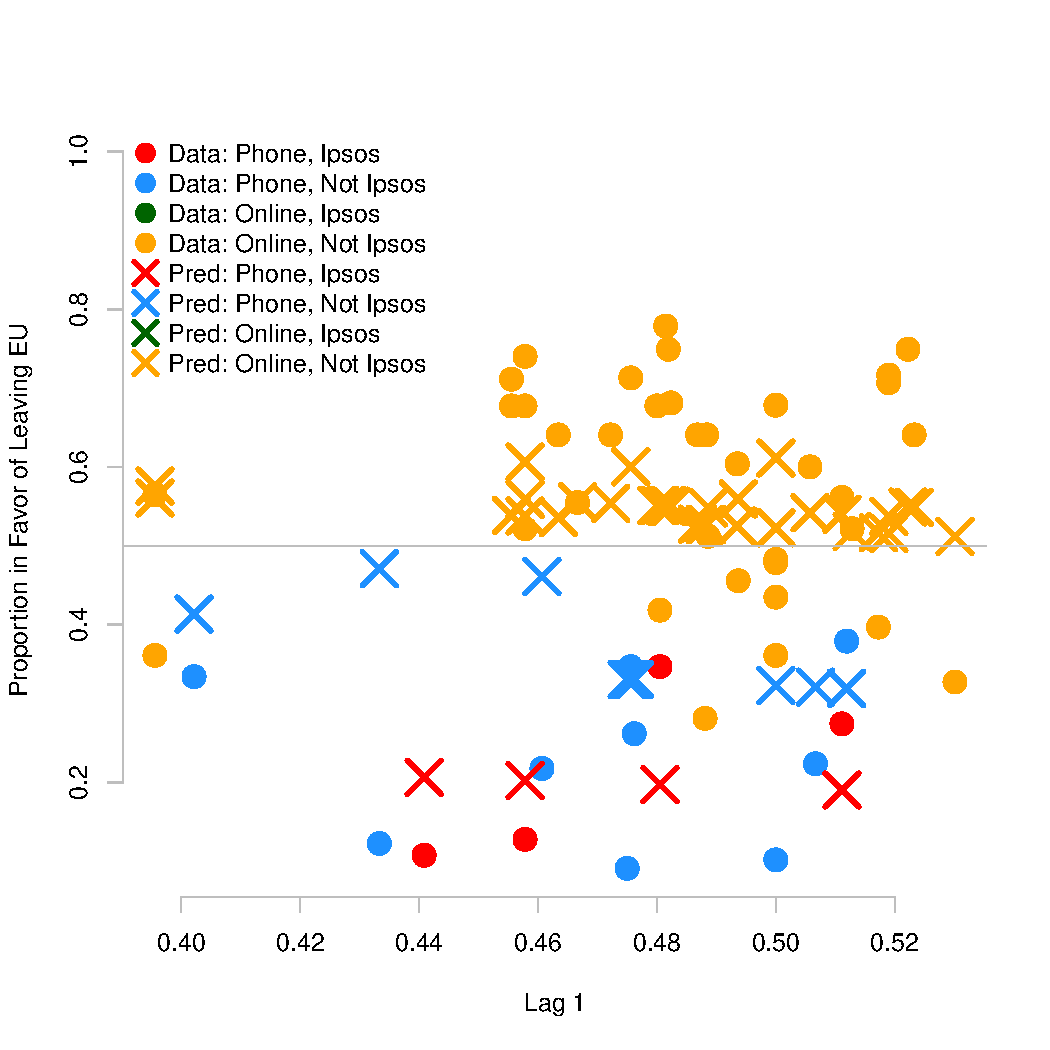
\includegraphics[scale=.5]{figs/preds.pdf}
  \caption{\small }
  \label{fig:allposts}
\end{figure}

\section{Methods}
\section{Analysis}
\section{Conclusions}

\begin{references}
{\footnotesize
\itemsep=3pt
\item {\em Park, T., \& Casella, G. (2008). The bayesian lasso. Journal of the American Statistical Association, 103(482), 681-686.}
\item {\em Gelman, A., Carlin, J. B., Stern, H. S., \& Rubin, D. B. (2014). Bayesian data analysis (Vol. 2). Boca Raton, FL, USA: Chapman \& Hall/CRC, 73.}
}

\end{references}
\end{document}

%\begin{figure*}
%  \centering
%  \includegraphics[scale=.55]{figs/mapDat.pdf}
%  \vspace{-7em}
%  \caption{\small Some Caption.}
%  \label{fig:mapDat}
%\end{figure*}

%\begin{figure}[H]
%  \includegraphics[scale=.5]{figs/pairsLogRate.pdf}
%  \caption{\small Hi Motor vehicle theft is not strongly correlated with any other thefts.}
%  \label{fig:logOdds}
%\end{figure}
